% !TEX program = pdflatex
% MDPI Drones submission draft.  The Definitions/ directory is the MDPI class
% bundle; replace author metadata and re-check the journal Instructions before submission.
% Tectonic uses XeTeX locally; Overleaf can compile the same source with pdfLaTeX
% by restoring the `pdftex` class option if desired.
\documentclass[drones,article,submit,moreauthors]{Definitions/mdpi}

\firstpage{1}
\makeatletter
\setcounter{page}{\@firstpage}
\makeatother
\pubvolume{1}
\issuenum{1}
\articlenumber{0}
\pubyear{2026}
\copyrightyear{2026}
\datereceived{}
\daterevised{}
\dateaccepted{}
\datepublished{}

\usepackage{amsmath,amssymb}
\usepackage{booktabs}
\usepackage{tabularx}
\usepackage{array}
\usepackage{enumitem}
\usepackage{xcolor}
\usepackage{graphicx}
\setlength{\headheight}{24pt}

\newcommand{\method}{Risk-Switch Lite-GLOBE-P}
\newcommand{\globe}{GLOBE-ROUTING}
\newcommand{\todo}[1]{\textcolor{red}{[TODO: #1]}}
\newcommand{\pdr}{\mathrm{PDR}}
\newcommand{\drop}{\mathrm{DROP}}
\newcolumntype{Y}{>{\centering\arraybackslash}X}
\newcommand{\scenario}[1]{\texttt{\seqsplit{#1}}}

\Title{Risk-Switch Lite-GLOBE-P: Global-to-Local Policy Distillation with Predictive Recovery for Decentralized FANET Routing}

\Author{First Author $^{1}$, Second Author $^{1}$ and Third Author $^{1}$*}
\AuthorNames{First Author, Second Author and Third Author}
\address{%
$^{1}$ \quad Department of Electrical and Computer Engineering, Institution, City, Republic of Korea; first.author@example.edu (F.A.); second.author@example.edu (S.A.)}
\corres{Correspondence: third.author@example.edu}

\abstract{%
Flying ad hoc networks (FANETs) must forward packets while their topology, link quality, and connectivity change rapidly. A routing policy that depends on a global graph or frequent inter-UAV messages is difficult to deploy at every relay. We present \method{}, a deployment-oriented routing framework that separates training-time privileged information from execution-time local information. A graph-aware PPO teacher is trained with the global topology, and its masked next-hop preferences are distilled into a compact student whose observation is restricted to the current relay, one-hop neighbors, link state, packet state, and bounded forwardability features. The student uses a geographic residual branch for ordinary states and a predictive branch for links with low margin, short estimated lifetime, or unstable onward connectivity. A calibrated risk switch activates the predictive branch only when the nominal action is unsafe or a sufficiently safer candidate exists. Phase 12 evaluates five training seeds, 14 held-out and stress scenarios, and 200 episodes per scenario (84,000 episode rows in total). Across the 14-scenario aggregate, \method{} achieves the highest connected-pair packet delivery ratio (PDR, 0.905) and deadline-delivery ratio (0.838) among the compared methods. It also reduces policy input bytes relative to Predictive Geographic, Evo-QGeo, and DRAMA, while incurring a modest energy-proxy cost relative to DRAMA. Stress results show that the switch recovers the predecessor's failure on predictive-break scenarios, although a highly lossy predictive-break case remains weaker than Evo-QGeo. These results support global-to-local distillation with selective predictive recovery as a practical design point for decentralized FANET routing.}

\keyword{flying ad hoc network; UAV routing; reinforcement learning; policy distillation; geographic routing; predictive link lifetime; decentralized networking; risk switching}

\begin{document}

\section{Introduction}

Flying ad hoc networks (FANETs) connect rapidly moving aerial nodes without a fixed infrastructure. Their short-lived links, intermittent connectivity, and limited onboard resources make next-hop selection fundamentally different from routing in a slowly varying terrestrial network. A geographic rule has a small control footprint, but a greedy progress decision can enter a structural routing hole or select a link that is valid now and fails before the next forwarding opportunity.

Recent learning-based approaches use graph encoders, actor--critic optimization, multi-agent coordination, predictive link information, or joint trajectory and resource control \cite{Alam2024JTFR,Wu2026AoI,Shou2026Adaptive,Zhang2026LargeScale}. These methods establish that learned policies can improve delivery reliability, but they also reveal a deployment tension: the global state, message exchange, or cross-layer variables used to learn a strong policy may not be available at every relay. A policy that cannot be evaluated from the information available at the forwarding node is not a decentralized routing policy in the strict sense.

This paper studies whether privileged global routing knowledge can be compressed into a strict one-hop policy and then complemented by a selective recovery mechanism. The proposed framework, \method, has three design principles. First, a global graph policy is used only as an offline teacher. Second, the deployed student is constrained to a masked one-hop action set and combines a geographic prior with a learned residual. Third, a predictive branch is evaluated only under a calibrated risk condition, so ordinary forwarding does not always pay the cost of the full predictive feature set.

The contributions are as follows:
\begin{enumerate}[leftmargin=*]
    \item We define a training/deployment separation for FANET routing in which a privileged global PPO teacher supervises a strict-local actor without online teacher communication.
    \item We introduce masked global-to-local policy distillation with geographic residual learning and forwardability features for recovery from structural routing holes.
    \item We design a predictive risk switch that uses local link margin, estimated link lifetime, queue headroom, and onward stability to invoke predictive recovery selectively.
    \item We provide a reproducible Phase 12 evaluation over five training seeds, 14 scenarios, 200 episodes per scenario, and six routing policies, reporting reliability, deadline delivery, tail delay, energy proxy, and policy input bytes together.
\end{enumerate}

The remainder of this paper is organized as follows. Section~2 reviews related FANET routing work. Section~3 formulates the local forwarding problem. Section~4 describes the proposed framework. Section~5 details the Phase 12 experimental protocol. Section~6 reports the results, Section~7 discusses implications and limitations, and Section~8 concludes the paper.

\section{Related Work}

\subsection{Learning-Based FANET Routing}

Value-based and actor--critic methods have been used to learn next-hop selection under mobility, interference, and traffic variation. Predictive-Q routing combines mobility and interference information with dual-path redundancy \cite{Dong2026Predictive}, while graph-attention Double DQN captures temporal and structural context \cite{Zhang2025Spatiotemporal}. Ultra-high-speed FANET routing demonstrates the importance of rapid topology adaptation \cite{Shou2026Adaptive}. These works motivate learning-based routing, but do not address the specific contract considered here: global information during training and one-hop information during deployment.

\subsection{Joint and Multi-Agent Optimization}

Joint trajectory, frequency allocation, and routing optimizes a broader cross-layer action space \cite{Alam2024JTFR}. AoI-aware sampling--buffering--routing further couples application freshness with network control \cite{Wu2026AoI}. Trusted routing adds security and blockchain-assisted trust to multi-agent forwarding \cite{Jia2025Trusted}. Such objectives are complementary to our focus on forwarding reliability under a small local observation. In contrast to message-passing multi-agent policies, the deployed \method{} does not require a global critic or online coordination channel.

\subsection{Deployment-Oriented Routing}

RoutePPO connects PPO-based decisions to Linux/eBPF forwarding \cite{Curmen2026RoutePPO}, providing an important deployment reference. Its path-selection setting differs from topology-varying, per-hop neighbor selection. Large-scale TVT work evaluates hundreds of UAVs \cite{Zhang2026LargeScale}; our contribution is instead the explicit measurement of the global-information-to-local-execution trade-off and the cost of selective predictive recovery.

\section{System Model and Problem Formulation}

At decision time $t$, the FANET is represented by a time-varying graph $\mathcal{G}_t=(\mathcal{V},\mathcal{E}_t)$. When a packet for destination $d$ is held by relay $u$, the valid action set is
\begin{equation}
    \mathcal{A}_u(t)=\mathcal{N}_u(t)\cup\{\drop\},
    \label{eq:action}
\end{equation}
where $\mathcal{N}_u(t)$ is the set of currently reachable one-hop neighbors. A structural mask removes disconnected and padded candidates. The explicit $\drop$ action represents a controlled discard when forwarding is unsafe or impossible; it prevents the policy from treating an invalid candidate as a valid relay.

The teacher observes a privileged state $s_t$ containing the global graph, node states, current relay, destination, and packet state. The deployed student observes only
\begin{equation}
o_u(t)=\left\{x_u(t),\{x_i(t)\}_{i\in\mathcal{N}_u(t)},
\{x_{u,i}(t)\}_{i\in\mathcal{N}_u(t)},x_d(t),x_p(t)\right\},
\label{eq:local-observation}
\end{equation}
where $x_p(t)$ denotes packet and forwarding context. The central question is whether a local policy $\pi_S(a\mid o_u)$ can retain useful preferences from $\pi_T(a\mid s_t)$ without receiving $s_t$ or messages from a centralized controller during execution.

\section{Proposed Method: \method}

\subsection{Privileged Global Teacher}

The offline teacher uses a graph encoder and actor--critic PPO. Its action logits are masked by the same relay-local support as the student, so distillation transfers a valid next-hop preference rather than an invalid global action. The clipped PPO objective is
\begin{equation}
\mathcal{L}_{\mathrm{PPO}}=-\mathbb{E}_t\left[\min\left(\rho_t A_t,\operatorname{clip}(\rho_t,1-\epsilon,1+\epsilon)A_t\right)\right],
\label{eq:ppo}
\end{equation}
where $\rho_t$ is the policy ratio and $A_t$ is the estimated advantage. The teacher is a training reference, not a deployment component and not assumed to be an optimal oracle.

\subsection{Masked Global-to-Local Distillation}

Teacher and student logits are restricted by the same action mask. With temperature $T$, the principal distillation term is
\begin{equation}
\mathcal{L}_{\mathrm{KD}}=T^2D_{\mathrm{KL}}\left(\pi_T^T(\cdot\mid s_t)\,\|\,\pi_S^T(\cdot\mid o_u)\right).
\label{eq:kd}
\end{equation}
The implementation also supports teacher-action, shortest-path-oracle, and risk-aware-oracle cross-entropy terms. Dataset partitions are made by scenario and episode seed rather than individual hops, preventing trajectory leakage between training and evaluation.

\subsection{Normal Geographic-Residual Branch}

For candidate $i$, $g_i$ denotes normalized progress toward the destination and $r_\theta(o_u,i)$ is a shared local MLP residual. The nominal logit is
\begin{equation}
z_i^N=\alpha g_i+r_\theta(o_u,i),
\label{eq:normal}
\end{equation}
with a forwardability feature and visited-action mask to reduce loops and greedy dead ends. This branch is deliberately lightweight and is the default in ordinary states.

\subsection{Predictive Risk Branch}

The predictive branch uses four bounded local features per candidate,
\begin{equation}
x_i^{\mathrm{risk}}=[m_i,\ell_i,q_i,o_i],
\label{eq:risk-features}
\end{equation}
where $m_i$ is link margin, $\ell_i$ is estimated current-link lifetime, $q_i$ is queue headroom, and $o_i$ is the predicted lifetime of the best onward link. Its danger score is
\begin{equation}
D_i=[\gamma_m-m_i]_+ + [\gamma_\ell-\ell_i]_+ + [\gamma_o-o_i]_+.
\label{eq:danger}
\end{equation}
The predictive prior and bounded residual favor candidates with sufficient progress, forwardability, and future connectivity while penalizing gate violations.

\subsection{Calibrated Risk Switching}

Let $a_N$ be the nominal action and $a_P$ the predictive-prior action. The predictive branch is selected when the nominal action is $\drop$, its danger exceeds a calibrated threshold $\tau$, or the predictive candidate has a safety gain greater than $\delta=0.10$ and a lower danger score:
\begin{equation}
S=\mathbb{1}\left[a_N=\drop\;\lor\;D_{a_N}>\tau\;\lor\;\left(a_P\neq a_N\land G(a_P,a_N)>0.10\land D_{a_P}<D_{a_N}\right)\right].
\label{eq:switch}
\end{equation}
The final action is $a_P$ when $S=1$ and $a_N$ otherwise. Calibration searches switch thresholds and margin, lifetime, and onward gates while requiring the general and structural-hole PDR not to fall more than 0.005 below the nominal reference. This makes the recovery mechanism selective rather than permanently predictive.

\subsection{Expected Deployment Trade-Off}

The method does not claim universal dominance. Predictive recovery can increase path length and energy proxy because it avoids a short but unstable link. Conversely, always running the predictive branch increases policy input bytes. The scientific claim is therefore a Pareto-style deployment trade-off: retain high delivery reliability and deadline delivery while reducing the information footprint relative to predictive and message-passing baselines.

\section{Experimental Design}

\subsection{Implementation and Evaluation Protocol}

Phase 12 uses the Lite-GLOBE simulator with CUDA training where available. Five training seeds (42, 77, 123, 314, and 2718) are evaluated over 14 scenario instances with 200 episodes per scenario. The resulting archive contains 84,000 episode rows, 420 seed-summary rows, 1,764 metric-statistic rows, and 280 paired-effect rows. All methods use the same action mask, episode budget, and scenario definitions.

The compared policies are GPSR, Predictive Geographic, Phase 8 Geo-Residual KD, Lite-GLOBE-P predictive-prior only, Lite-GLOBE-P no-switch, and the proposed Risk-Switch Lite-GLOBE-P. The primary reliability metric is connected-pair PDR. Secondary metrics are deadline-delivery ratio, p95 successful delay, transmission-energy proxy, and policy input bytes. Delay and cost metrics are interpreted jointly with delivery metrics because a policy that drops early can appear artificially fast.

\subsection{Scenario Groups and Research Questions}

The 14 scenarios cover held-out medium mobility, link loss, fast and extreme mobility, sparse connectivity, node-count shifts (10, 16, and 24 nodes), structural routing holes, predictive link breaks, and link-loss stress. We ask:
\begin{enumerate}[leftmargin=*]
    \item Does distillation improve strict-local reliability over geographic routing and the Phase 8 predecessor?
    \item Does the switch preserve ordinary-state performance while recovering predictive-break failures?
    \item Does selective prediction reduce input bytes relative to always-on predictive baselines?
    \item Which reliability gains are accompanied by delay or energy trade-offs?
\end{enumerate}

\subsection{Reproducibility and Statistical Treatment}

The release stores raw episode records, seed summaries, aggregate statistics, paired effects, configuration, and generated figures. Means in the tables are aggregated over the 14 scenario means. The seed-paired comparison is the preferred inferential unit; no smoke results are mixed with the full Phase 12 archive. Because several deterministic scenarios produce zero empirical variance, the descriptive tables show the exact aggregate means and the companion paired-effects archive should be used for uncertainty intervals.

\section{Results}

\subsection{Aggregate Performance}

Table~\ref{tab:overall} reports the 14-scenario aggregate. \method{} obtains the highest PDR and deadline-delivery ratio among the compared policies. Its p95 delay is lower than the predictive geographic, Evo-QGeo, and DRAMA references summarized in the Phase 12 analysis, while Phase 8 remains slightly faster in the aggregate. Input bytes are 12.8\% lower than Predictive Geographic, 25.3\% lower than Evo-QGeo, and 22.7\% lower than DRAMA. The energy proxy is 3.2\% higher than DRAMA and 25.0\% higher than Phase 8, reflecting safer but sometimes longer routes.

\begin{table}[H]
\caption{Phase 12 aggregate over 14 scenarios. Values are means over scenario-level summaries.}
\label{tab:overall}
\centering
\small
\begin{tabularx}{\textwidth}{lYYYYY}
\toprule
Method & PDR & Deadline & p95 delay & Energy proxy & Input bytes \\
\midrule
GPSR & 0.683 & 0.637 & 4.163 & 1.166 & 2284 \\
Predictive Geographic & 0.892 & 0.823 & 4.500 & 1.809 & 5531 \\
Evo-QGeo & 0.887 & 0.815 & 4.557 & 1.812 & 6452 \\
IQMR Q($\lambda$) & 0.516 & 0.385 & 6.289 & 1.946 & 7953 \\
DRAMA & 0.891 & 0.822 & 4.504 & 1.724 & 6240 \\
Phase 8 Geo-Residual KD & 0.803 & 0.740 & 4.110 & 1.424 & 3956 \\
Predictive-prior only & 0.905 & 0.838 & 4.334 & 1.776 & 5424 \\
No-switch & 0.890 & 0.822 & 4.300 & 1.726 & 5775 \\
\textbf{\method} & \textbf{0.905} & \textbf{0.838} & \textbf{4.264} & 1.779 & \textbf{4821} \\
\bottomrule
\end{tabularx}
\end{table}

Figures~\ref{fig:pdr}--\ref{fig:input} visualize the same full 14-scenario archive. The PDR curve shows the defining behavior of the switch: the proposed method stays near the strongest methods in ordinary and node-shift scenarios, while avoiding the near-zero PDR of the Phase 8 predecessor on predictive-break cases. The delay curve makes the cost of recovery visible, and the input-byte curve shows that selective activation is lighter than always-on predictive policies in most scenarios.

\begin{figure}[H]
\centering
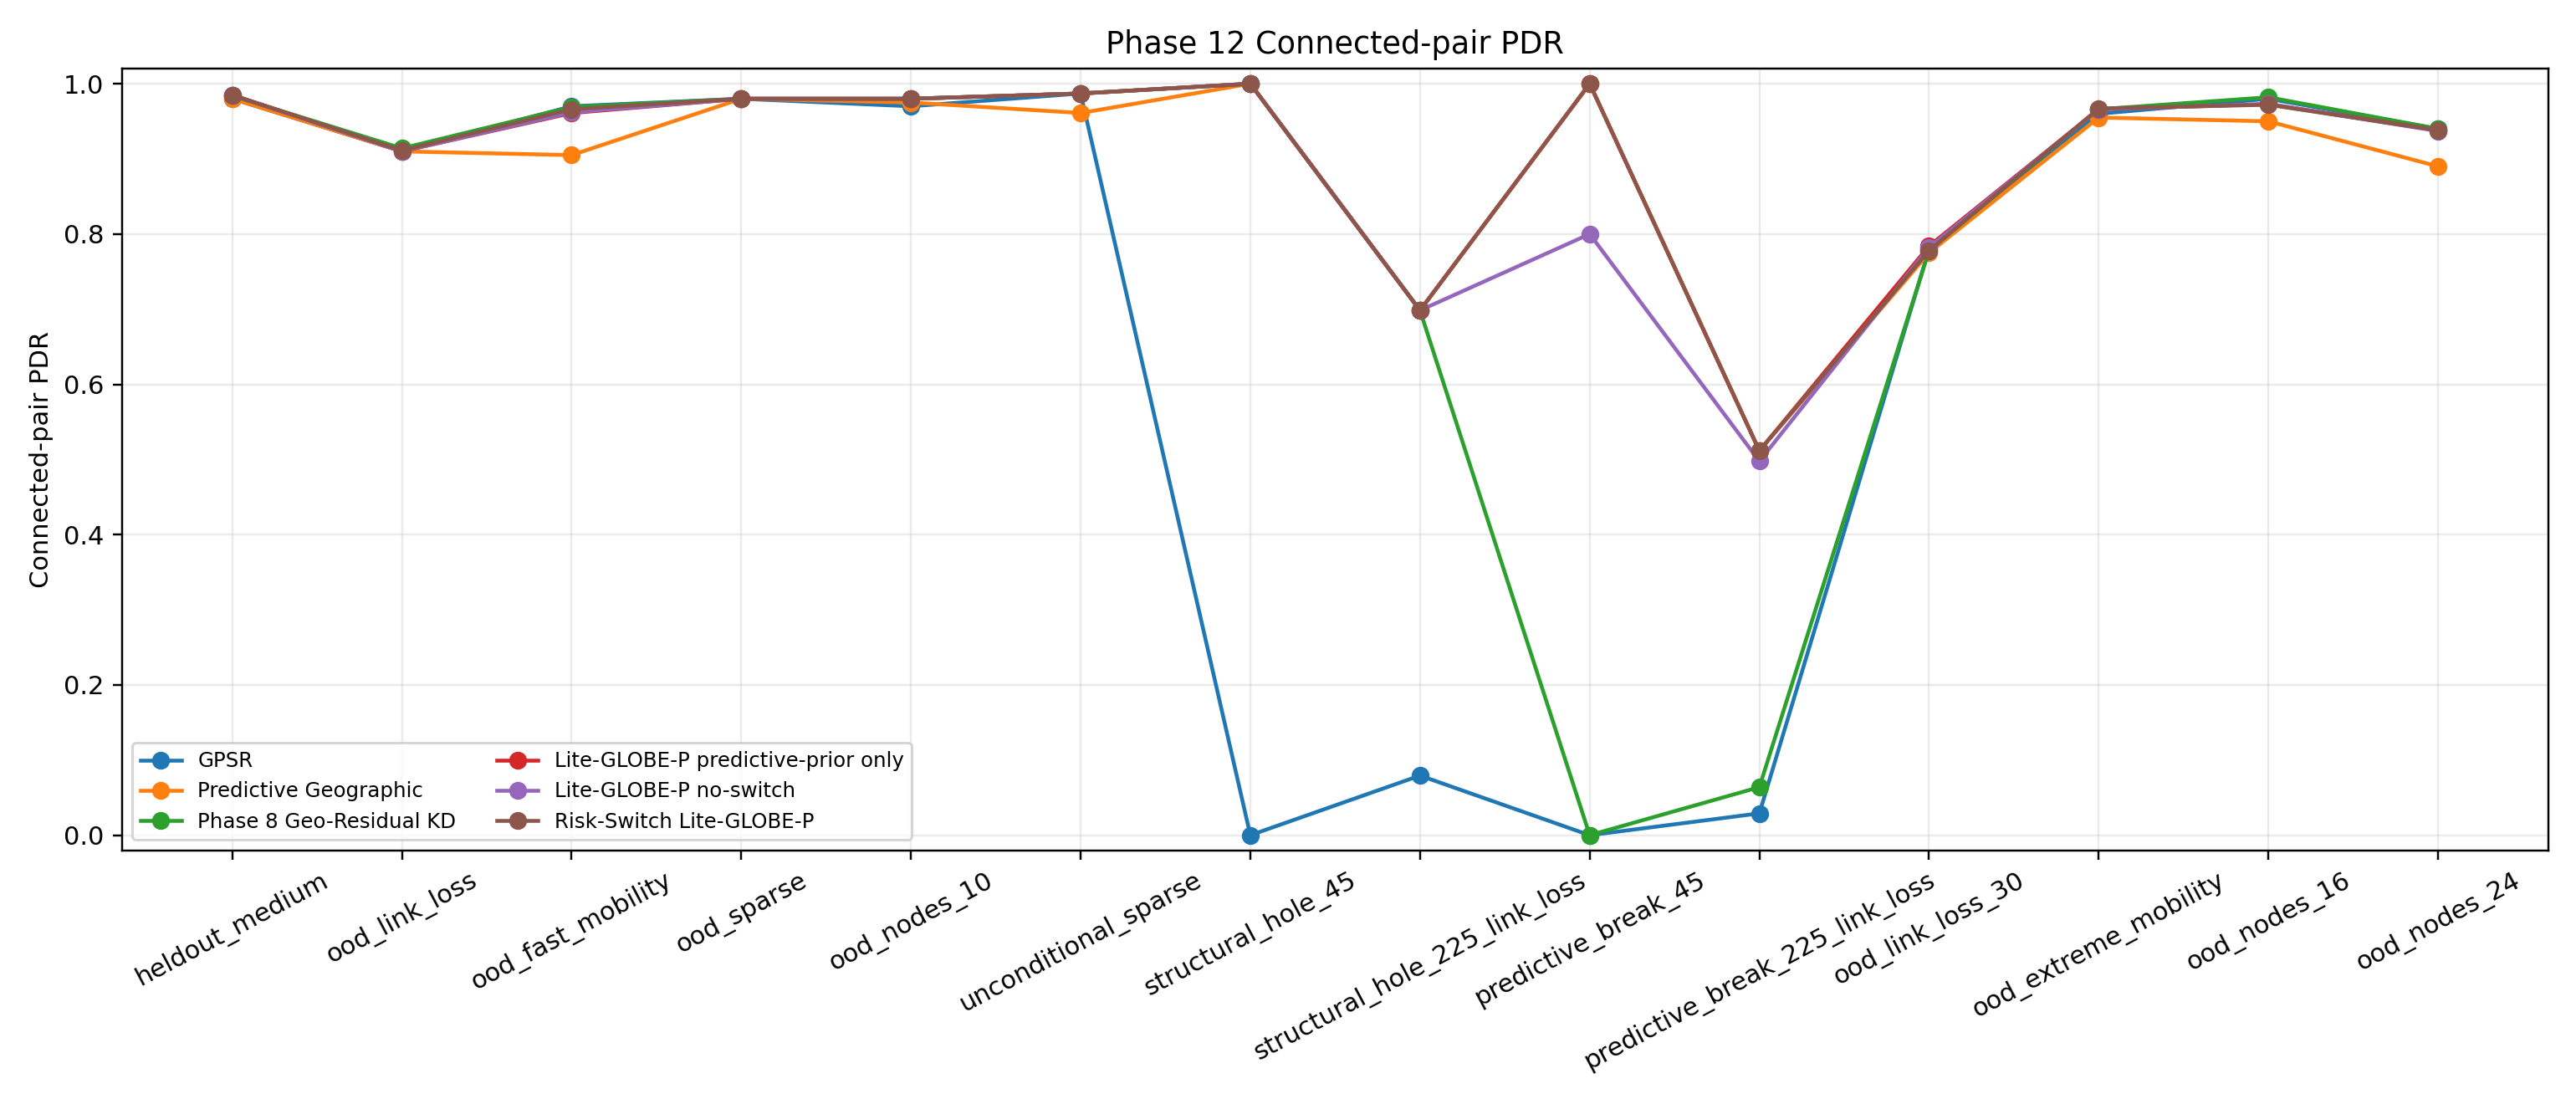
\includegraphics[width=\textwidth]{figures/phase12_pdr.png}
\caption{Connected-pair PDR across all 14 Phase 12 scenarios. Risk-Switch Lite-GLOBE-P combines the normal branch in benign states with predictive recovery in unstable states.}
\label{fig:pdr}
\end{figure}

\begin{figure}[H]
\centering
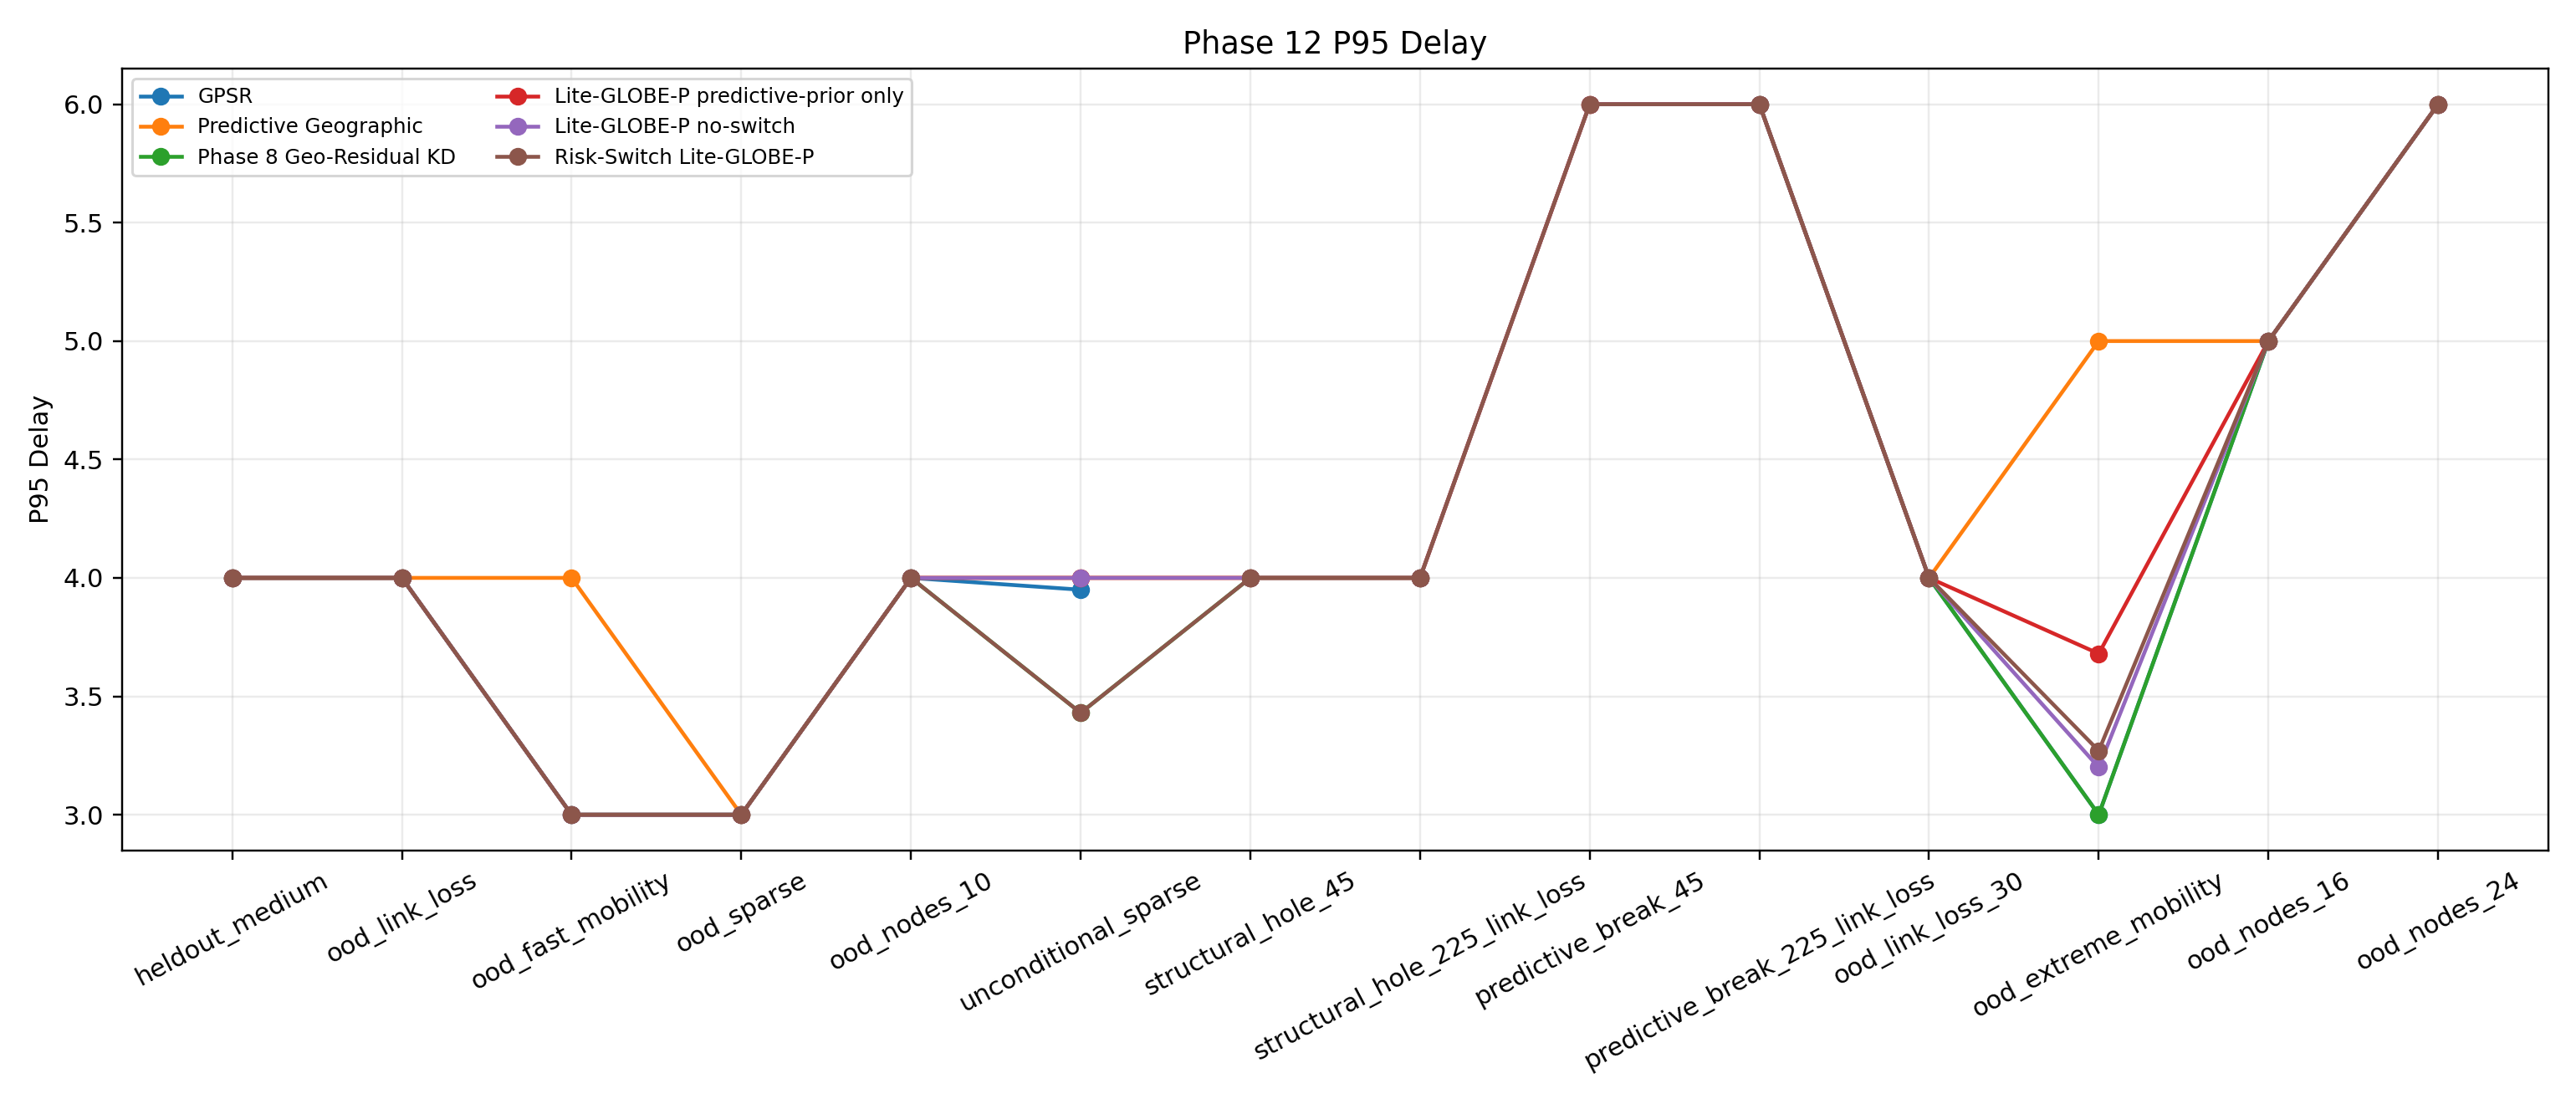
\includegraphics[width=\textwidth]{figures/phase12_delay_p95.png}
\caption{95th-percentile successful delay across Phase 12 scenarios. Higher delay in recovery cases reflects continued forwarding along safer alternatives rather than early failure.}
\label{fig:delay}
\end{figure}

\begin{figure}[H]
\centering
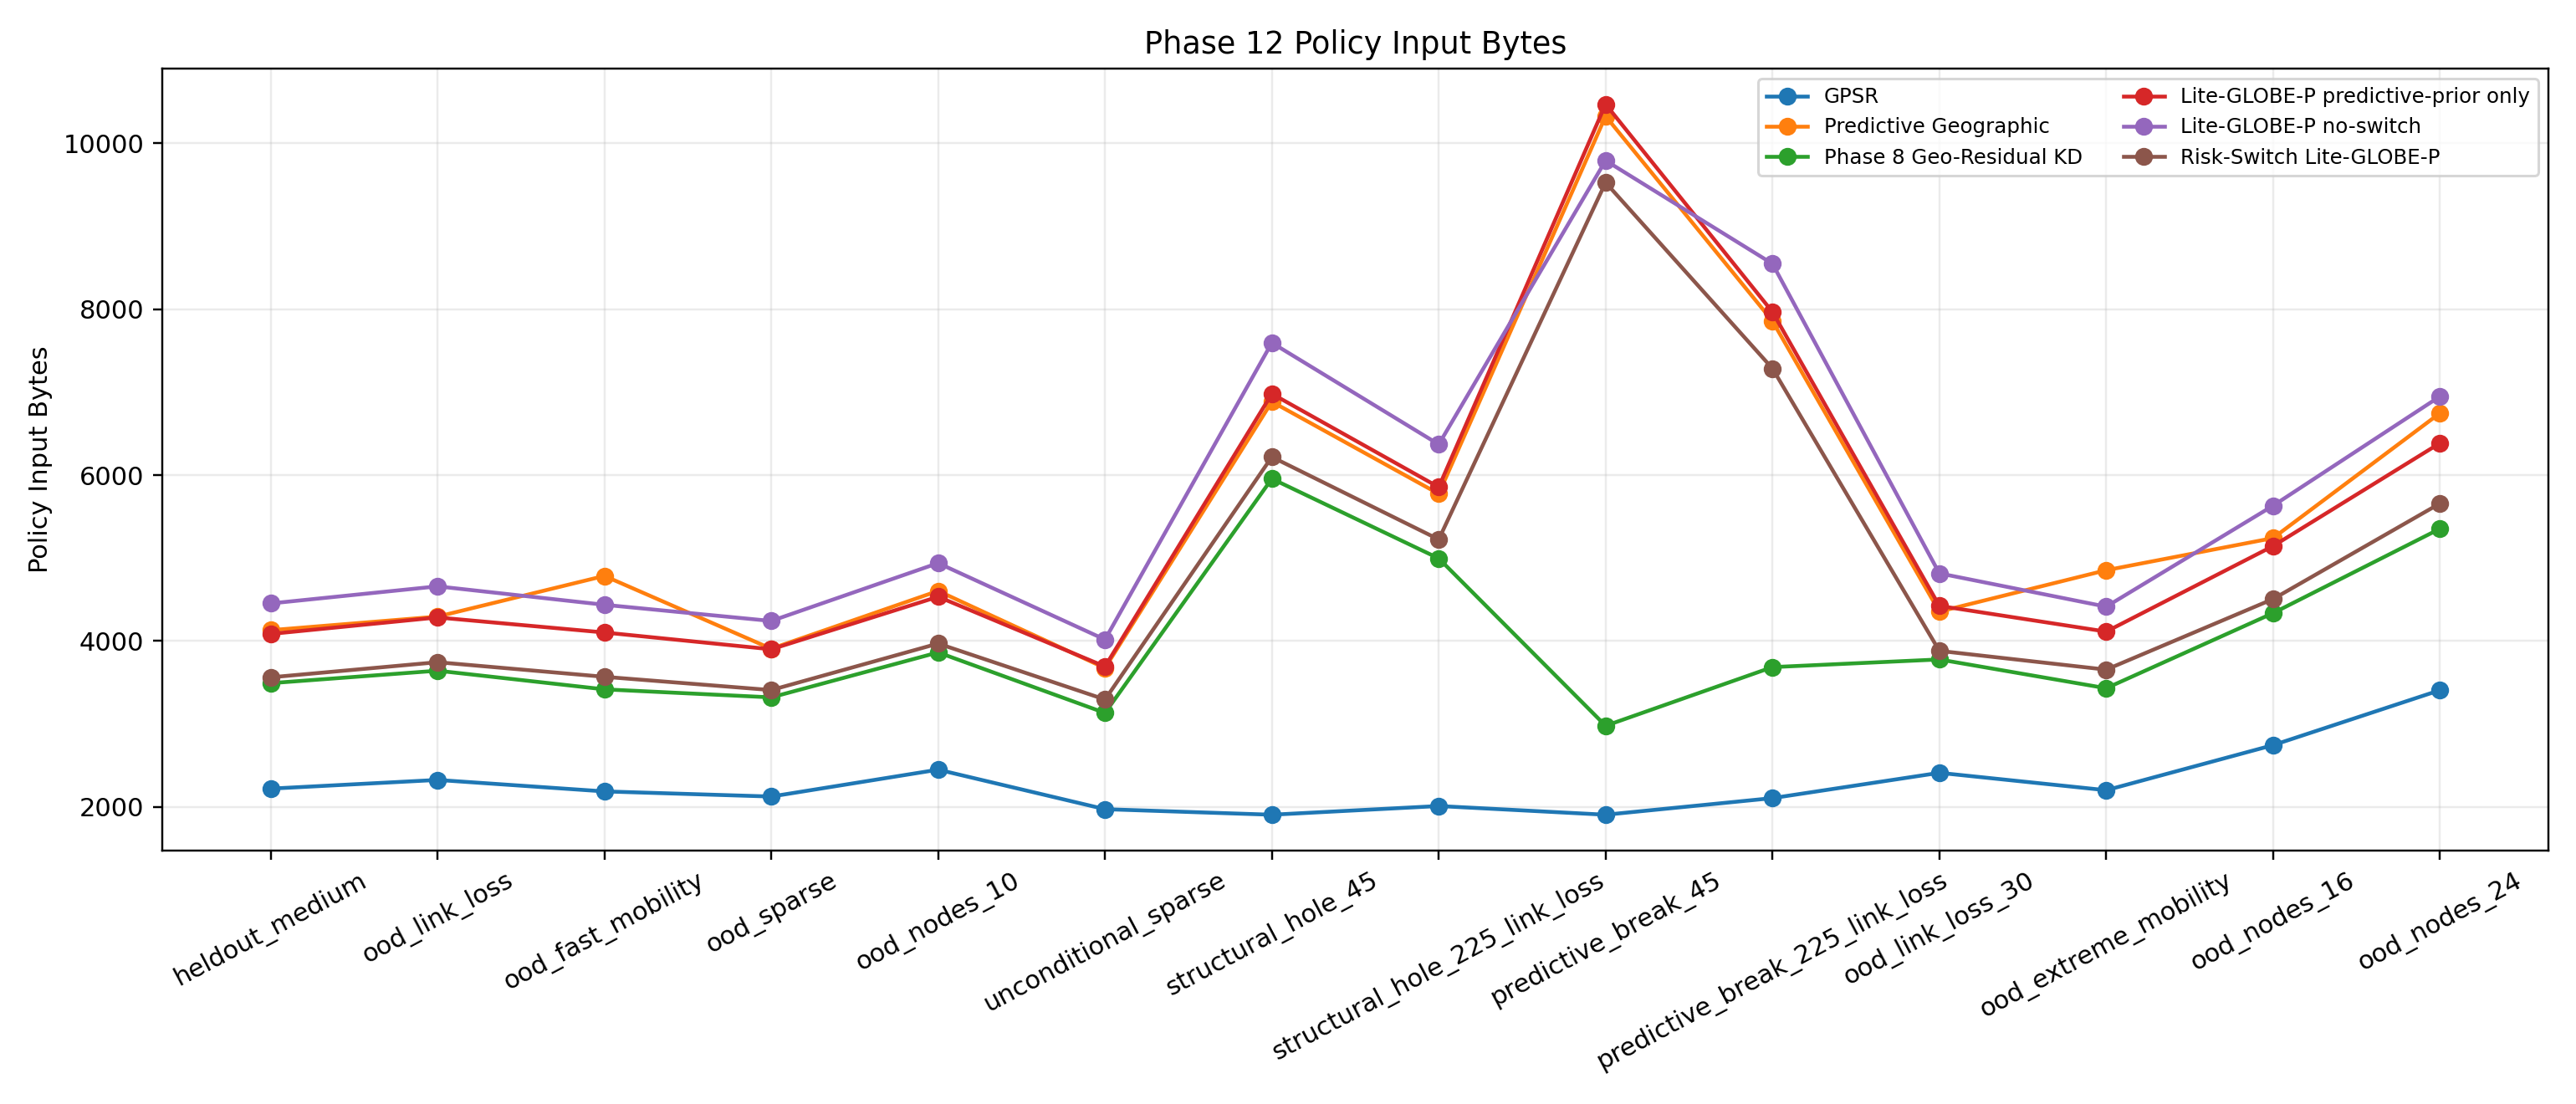
\includegraphics[width=\textwidth]{figures/phase12_input_bytes.png}
\caption{Policy input bytes across Phase 12 scenarios. Selective switching reduces the information footprint relative to always-on predictive and no-switch policies.}
\label{fig:input}
\end{figure}

\subsection{Structural-Hole and Predictive-Break Stress Tests}

Table~\ref{tab:stress} isolates the scenarios that motivated the method. In the rotated structural-hole case, GPSR fails completely while all learned recovery policies reach PDR 1.000. In the clean predictive-break case, Phase 8 again collapses to PDR 0.000, whereas \method{} reaches 1.000. Under predictive break combined with link loss, \method{} reaches PDR 0.512, recovering the Phase 8 failure but remaining below Evo-QGeo's 0.558 in the more difficult comparison reported in the Phase 12 analysis.

\begin{table}[H]
\caption{Stress scenarios from Phase 12.}
\label{tab:stress}
\centering
\small
\begin{tabularx}{\textwidth}{lYYYY}
\toprule
Scenario and method & PDR & Deadline & p95 delay & Input bytes \\
\midrule
Structural hole 45, GPSR & 0.000 & 0.000 & N/A & 1906 \\
Structural hole 45, \method & 1.000 & 1.000 & 4.000 & 6218 \\
Predictive break 45, Phase 8 & 0.000 & 0.000 & N/A & 2978 \\
Predictive break 45, \method & 1.000 & 1.000 & 6.000 & 9526 \\
Break 225 + loss, Predictive Geographic & 0.512 & 0.440 & 6.000 & 7856 \\
Break 225 + loss, Evo-QGeo & 0.558 & 0.480 & 6.000 & 9100 \\
Break 225 + loss, \method & 0.512 & 0.440 & 6.000 & 7284 \\
\bottomrule
\end{tabularx}
\end{table}

\subsection{Node-Count Generalization and Cost Trade-Off}

On the three node-count shifts, \method{} obtains PDR 0.963, 0.972, and 0.938 for 10, 16, and 24 nodes, respectively. Phase 8 is slightly higher on the 10-node and 24-node aggregates (0.967 and 0.940), indicating that the risk branch is not a universal improvement under every density shift. The proposed method nevertheless remains above Predictive Geographic, Evo-QGeo, and DRAMA on the aggregate reliability comparison, with lower input bytes than those predictive baselines.

\section{Discussion}

\subsection{What the Results Establish}

The results support four bounded conclusions. First, global-to-local distillation can improve a strict-local policy over GPSR and the Phase 8 predecessor when evaluated across heterogeneous mobility and failure conditions. Second, the risk switch addresses the predecessor's central failure mode: a locally attractive link that is about to break. Third, selective activation lowers input information relative to always-on predictive and message-passing references. Fourth, reliability gains are not free: safe detours can increase energy proxy and p95 delay, and a highly lossy predictive-break case remains an open weakness.

The correct novelty claim is therefore architectural and deployment-oriented, not that PPO itself is new. The novelty lies in the explicit contract between privileged training and strict-local execution, masked transfer of global next-hop preferences, and a calibrated gate that invokes predictive recovery only when the nominal action is risky.

\subsection{Limitations and Threats to Validity}

The current evidence is simulator-level. The Lite-GLOBE environment abstracts physical and medium-access layers, uses simplified mobility, and reports an energy proxy rather than radio-power measurements. Input bytes measure policy feature input and should not be conflated with full protocol control-plane overhead. The present comparison also does not include a packet-level AODV or OLSR implementation, ns-3/OMNeT++ cross-validation, or live Linux/eBPF forwarding. Consequently, the results establish controlled routing-logic behavior, not flight-ready performance.

The Phase 12 archive is complete for the stated five-seed protocol, but it does not include the later Phase 13/P+ variants. Claims about redundancy, loss-keep, energy-tie, or DROP-suppression variants must not be attributed to this paper. Before submission, the authors should add protocol baselines, report seed-paired confidence intervals in the main tables, and validate the most important predictive-break result in a second network simulator or testbed.

\subsection{Reproducibility}

The experiment configuration, code paths, raw records, aggregate reports, and figure-generation scripts are versioned in the project repository. A release accompanying submission should archive the exact Phase 12 manifest, training seeds, evaluation seeds, and the generated tables and figures. This will allow reviewers to reproduce both the favorable aggregate result and the Evo-QGeo advantage in the lossy predictive-break case.

\section{Conclusions}

We presented \method, a global-to-local policy-distillation framework for decentralized FANET packet routing. A privileged global PPO teacher is used only offline; the deployed student operates on a masked one-hop observation and combines a geographic residual with a selectively activated predictive risk branch. In the Phase 12 full evaluation, the method achieves the best aggregate PDR (0.905) and deadline delivery (0.838) among the compared policies and reduces input bytes relative to predictive and message-passing references. The method also recovers structural-hole and clean predictive-break failures, at the cost of a modest energy and delay trade-off and with a remaining weakness under highly lossy predictive breaks. Future work will add protocol-stack baselines, radio-aware energy, cross-simulator validation, and larger-scale or hardware-in-the-loop experiments.

\authorcontributions{Conceptualization, First Author and Second Author; methodology, First Author and Second Author; software, First Author; validation, Second Author; formal analysis, First Author; investigation, First Author and Third Author; writing--original draft preparation, First Author; writing--review and editing, all authors; visualization, First Author; supervision, Third Author; project administration, Third Author.}
\funding{This research received no external funding. \todo{Confirm or replace with the exact funder and grant number.}}
\institutionalreview{Not applicable.}
\informedconsent{Not applicable.}
\dataavailability{The Phase 12 experiment archive, configuration, generated tables, and figures are available in the project repository. \todo{Insert the public repository URL and archived release DOI before submission.}}
\acknowledgments{The authors thank the project collaborators who contributed to the Lite-GLOBE experiment harness. \todo{Confirm names and support statements.}}
\conflictsofinterest{The authors declare no conflict of interest.}

\abbreviations{Abbreviations}{
\noindent
\begin{tabular}{@{}ll}
FANET & Flying Ad Hoc Network\\
GPSR & Greedy Perimeter Stateless Routing\\
PDR & Packet Delivery Ratio\\
PPO & Proximal Policy Optimization\\
KD & Knowledge Distillation
\end{tabular}}

\appendix
\section{Phase 12 Method and Scenario Inventory}

The six evaluated policies are GPSR, Predictive Geographic, Phase 8 Geo-Residual KD, Lite-GLOBE-P predictive-prior only, Lite-GLOBE-P no-switch, and Risk-Switch Lite-GLOBE-P. The 14 scenario names in the generated archive are listed below; the naming is retained to make the manuscript tables directly auditable against the Phase 12 report.
\begin{itemize}[leftmargin=*]
\item \scenario{heldout\_medium}, \scenario{ood\_link\_loss}, \scenario{ood\_fast\_mobility}, \scenario{ood\_sparse}, \scenario{ood\_nodes\_10}, \scenario{unconditional\_sparse}.
\item \scenario{structural\_hole\_45}, \scenario{structural\_hole\_225\_link\_loss}, \scenario{predictive\_break\_45}, \scenario{predictive\_break\_225\_link\_loss}.
\item \scenario{ood\_link\_loss\_30}, \scenario{ood\_extreme\_mobility}, \scenario{ood\_nodes\_16}, \scenario{ood\_nodes\_24}.
\end{itemize}

\bibliography{references}

\PublishersNote{}
\end{document}
